% Chapter Template

\chapter{Ensayos y Resultados} % Main chapter title

\label{Chapter4} % Change X to a consecutive number; for referencing this chapter elsewhere, use \ref{ChapterX}

%----------------------------------------------------------------------------------------
%	SECTION 1
%----------------------------------------------------------------------------------------

\section{Ensayos}
\label{sec:Ensayos}

Para verificar y validar la correcta implementación del sistema se procede a evaluar el funcionamiento aplicando técnicas de ensayos de caja negra.
%-----------------------------------
%	SUBSECTION 1
%-----------------------------------
%\subsection{Ensayos de caja blanca}

%Durante las primeras etapas de desarrollo del \textit{firmware} se hizo uso intensivo de las capacidades de \textit{debugging} a través de la interfaz JTAG

%-----------------------------------
%	SUBSECTION 2
%-----------------------------------

\subsection{Ensayos de caja negra}

Se utiliza la técnica de inyección de fallas para evaluar la respuesta del sistema frente a las distintas condiciones de alarma posibles.  El ensayo consiste en forzar las entradas de los sensores a valores que disparen las condiciones de alarma y contrastar las acciones de control del sistema con las esperadas.

Se utiliza la UART para realizar un seguimiento en el tiempo del valor de los sensores, del estado de las alarmas y del estado de los actuadores. Se tomaron muestras a una tasa de una muestra por segundo mientras se hacían variar las entradas del sistema para recorrer todas las posibles combinaciones de alarmas. La información fue procesada mediante rutinas de MATLAB elaboradas \textit{ad-hoc} para obtener gráficas del estado del sistema que permitieran corroborar su correcto funcionamiento. Los resultados se pueden observar en la sección \ref{sec:Resultados}. 

Si bien el sistema tiene seis condiciones de alarma, cada uno de los tres sensores tiene dos condiciones, una por exceso y otra por defecto, que son mutuamente excluyentes.  Por este motivo, el máximo número de alarmas simultáneas que puede haber en un momento dado es tres. Para analizar el comportamiento del sistema se agrupan las respuestas según la cantidad de alarmas en conjuntos de una única alarma, dos alarmas o tres alarmas simultáneas.

Para garantizar que se recorre todo el espacio de posibilidades de alarma se elaboran tablas de decisión con las acciones que se deben tomar para las distintas combinaciones posibles.  Se representa mediante una ``Y'' la condición de alarma presente.  En caso contrario se utiliza una ``N''. Las acciones de contingencia necesarias se indican con una ``X'' en el casillero correspondiente. Un casillero en blanco significa que esa acción en particular puede tener cualquiera de sus dos estados posibles sin que eso afecte la condición de alarma. 

Se muestra en el cuadro \ref{tab:1alarma} las acciones de contingencia para cuando hay una única condición de alarma en el sistema.  En el cuadro \ref{tab:2alarmas} se indican las acciones para las distintas combinaciones de dos alarmas. En el cuadro \ref{tab:3alarmas} se indican las acciones de contingencia para las combinaciones de tres alarmas.


\begin{table}[ht]
	\centering
	\caption{Tabla de decisión para el control de una sola alarma.}
    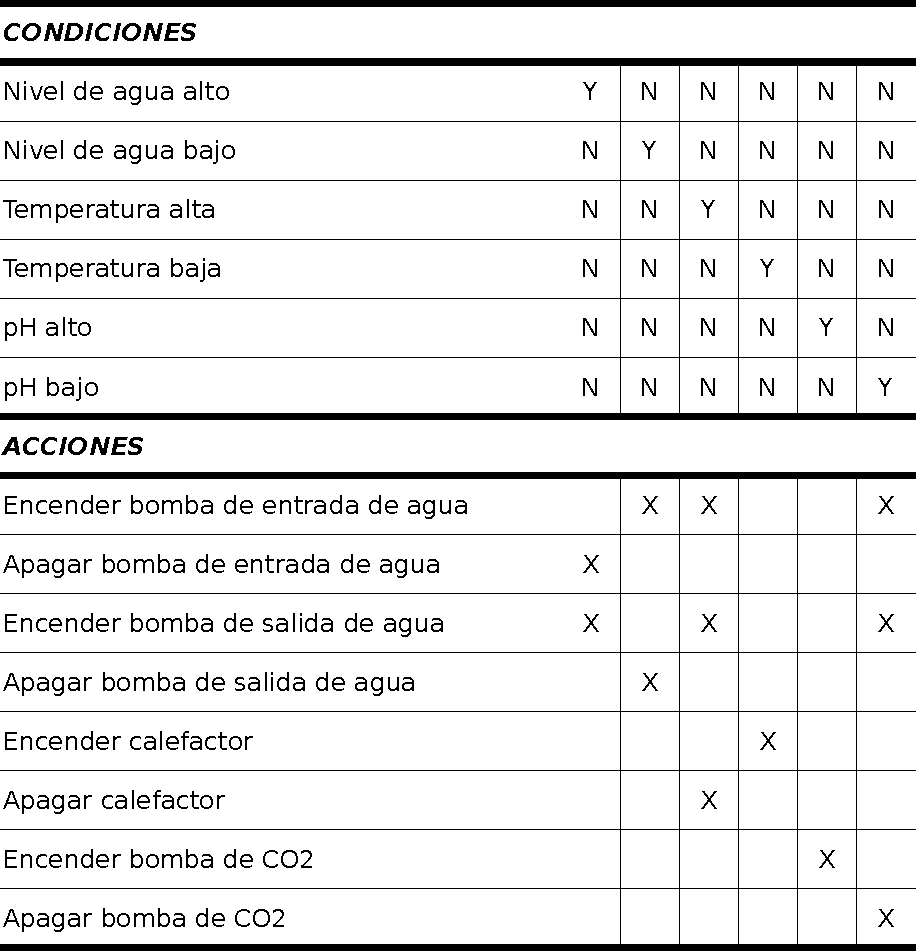
\includegraphics[height=.4\textheight]{./Figures/tabla1alarma.pdf}
	\label{tab:1alarma}
\end{table}

\begin{table}[ht]
\centering
\caption{Tabla de decisión para el control de dos alarmas.}
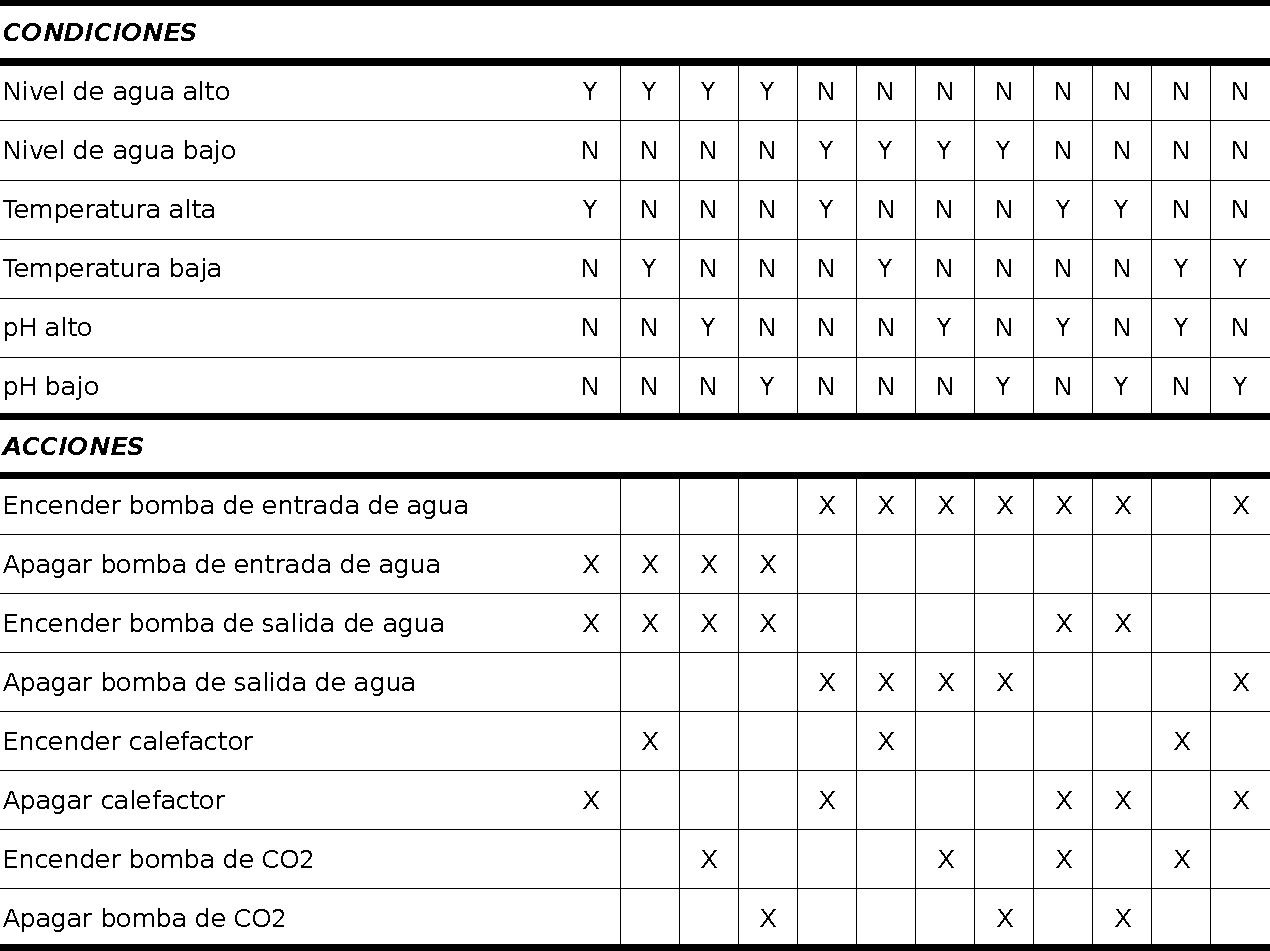
\includegraphics[height=.4\textheight]{./Figures/tabla2alarmas.pdf}
\label{tab:2alarmas}
\end{table}

\vspace{5px}

\begin{table}[htp!]
	\centering
	\caption{Tabla de decisión para el control de tres alarmas.}
    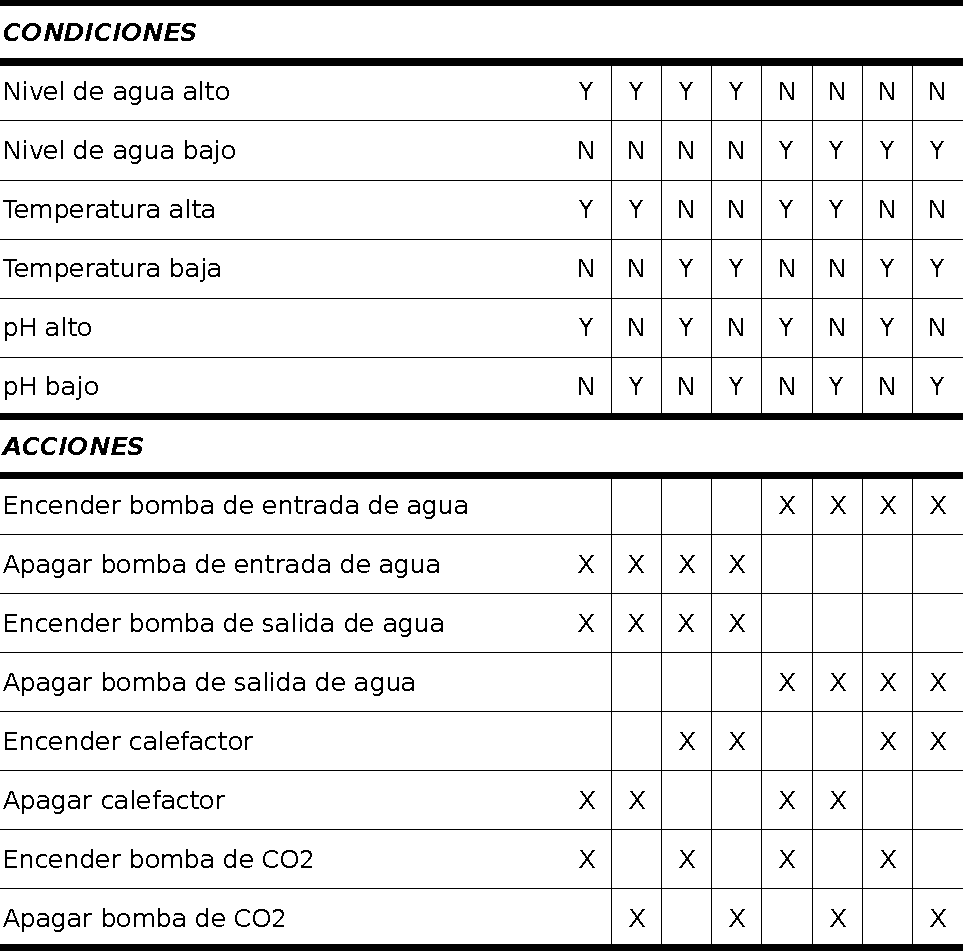
\includegraphics[height=.4\textheight]{./Figures/tabla3alarmas.pdf}
	\label{tab:3alarmas}
\end{table}

%----------------------------------------------------------------------------------------
%	SECTION 2
%----------------------------------------------------------------------------------------
\clearpage
\section{Resultados}
\label{sec:Resultados}

En esta sección se muestran los resultados correspondientes a las distintas combinaciones de alarmas presentes en el sistema.  Se puede observar el valor de los sensores junto con sus valores límite graficados en línea punteada y el estado lógico de los actuadores.  Por simplicidad de la gráfica, el estado de los actuadores de iluminación y bomba de $O_2$ no se muestran para ningún caso de análisis, ya que no tienen efecto sobre las condiciones de alarma.

Se agrupan los resultados con el criterio ya mencionado de cantidad de alarmas simultáneas.  En la sección \ref{sec:1alarma} se muestran los resultados para una única alarma presente. En la sección \ref{sec:2alarma} se pueden ver los resultados para dos alarmas presentes y finalmente, en la sección \ref{sec:3alarma} se encuentran los resultados para tres alarmas simultáneas.

\subsection{Respuesta a una única alarma}
\label{sec:1alarma}
Existen seis combinaciones de una única alarma, según fueron listadas en el cuadro \ref{tab:1alarma}. En la figura \ref{fig:alarma1nivel} se muestra la respuesta del sistema frente a las alarmas de nivel de agua alto y nivel de agua bajo . En la figura \ref{fig:alarma1Temp} se puede ver la respuesta frente a las alarmas de temperatura alta y temperatura baja. Finalmente, en la figura \ref{fig:alarma1pH} se grafica la respuesta frente a las alarmas de pH alto y pH bajo.

\begin{figure}[h]
\centering
    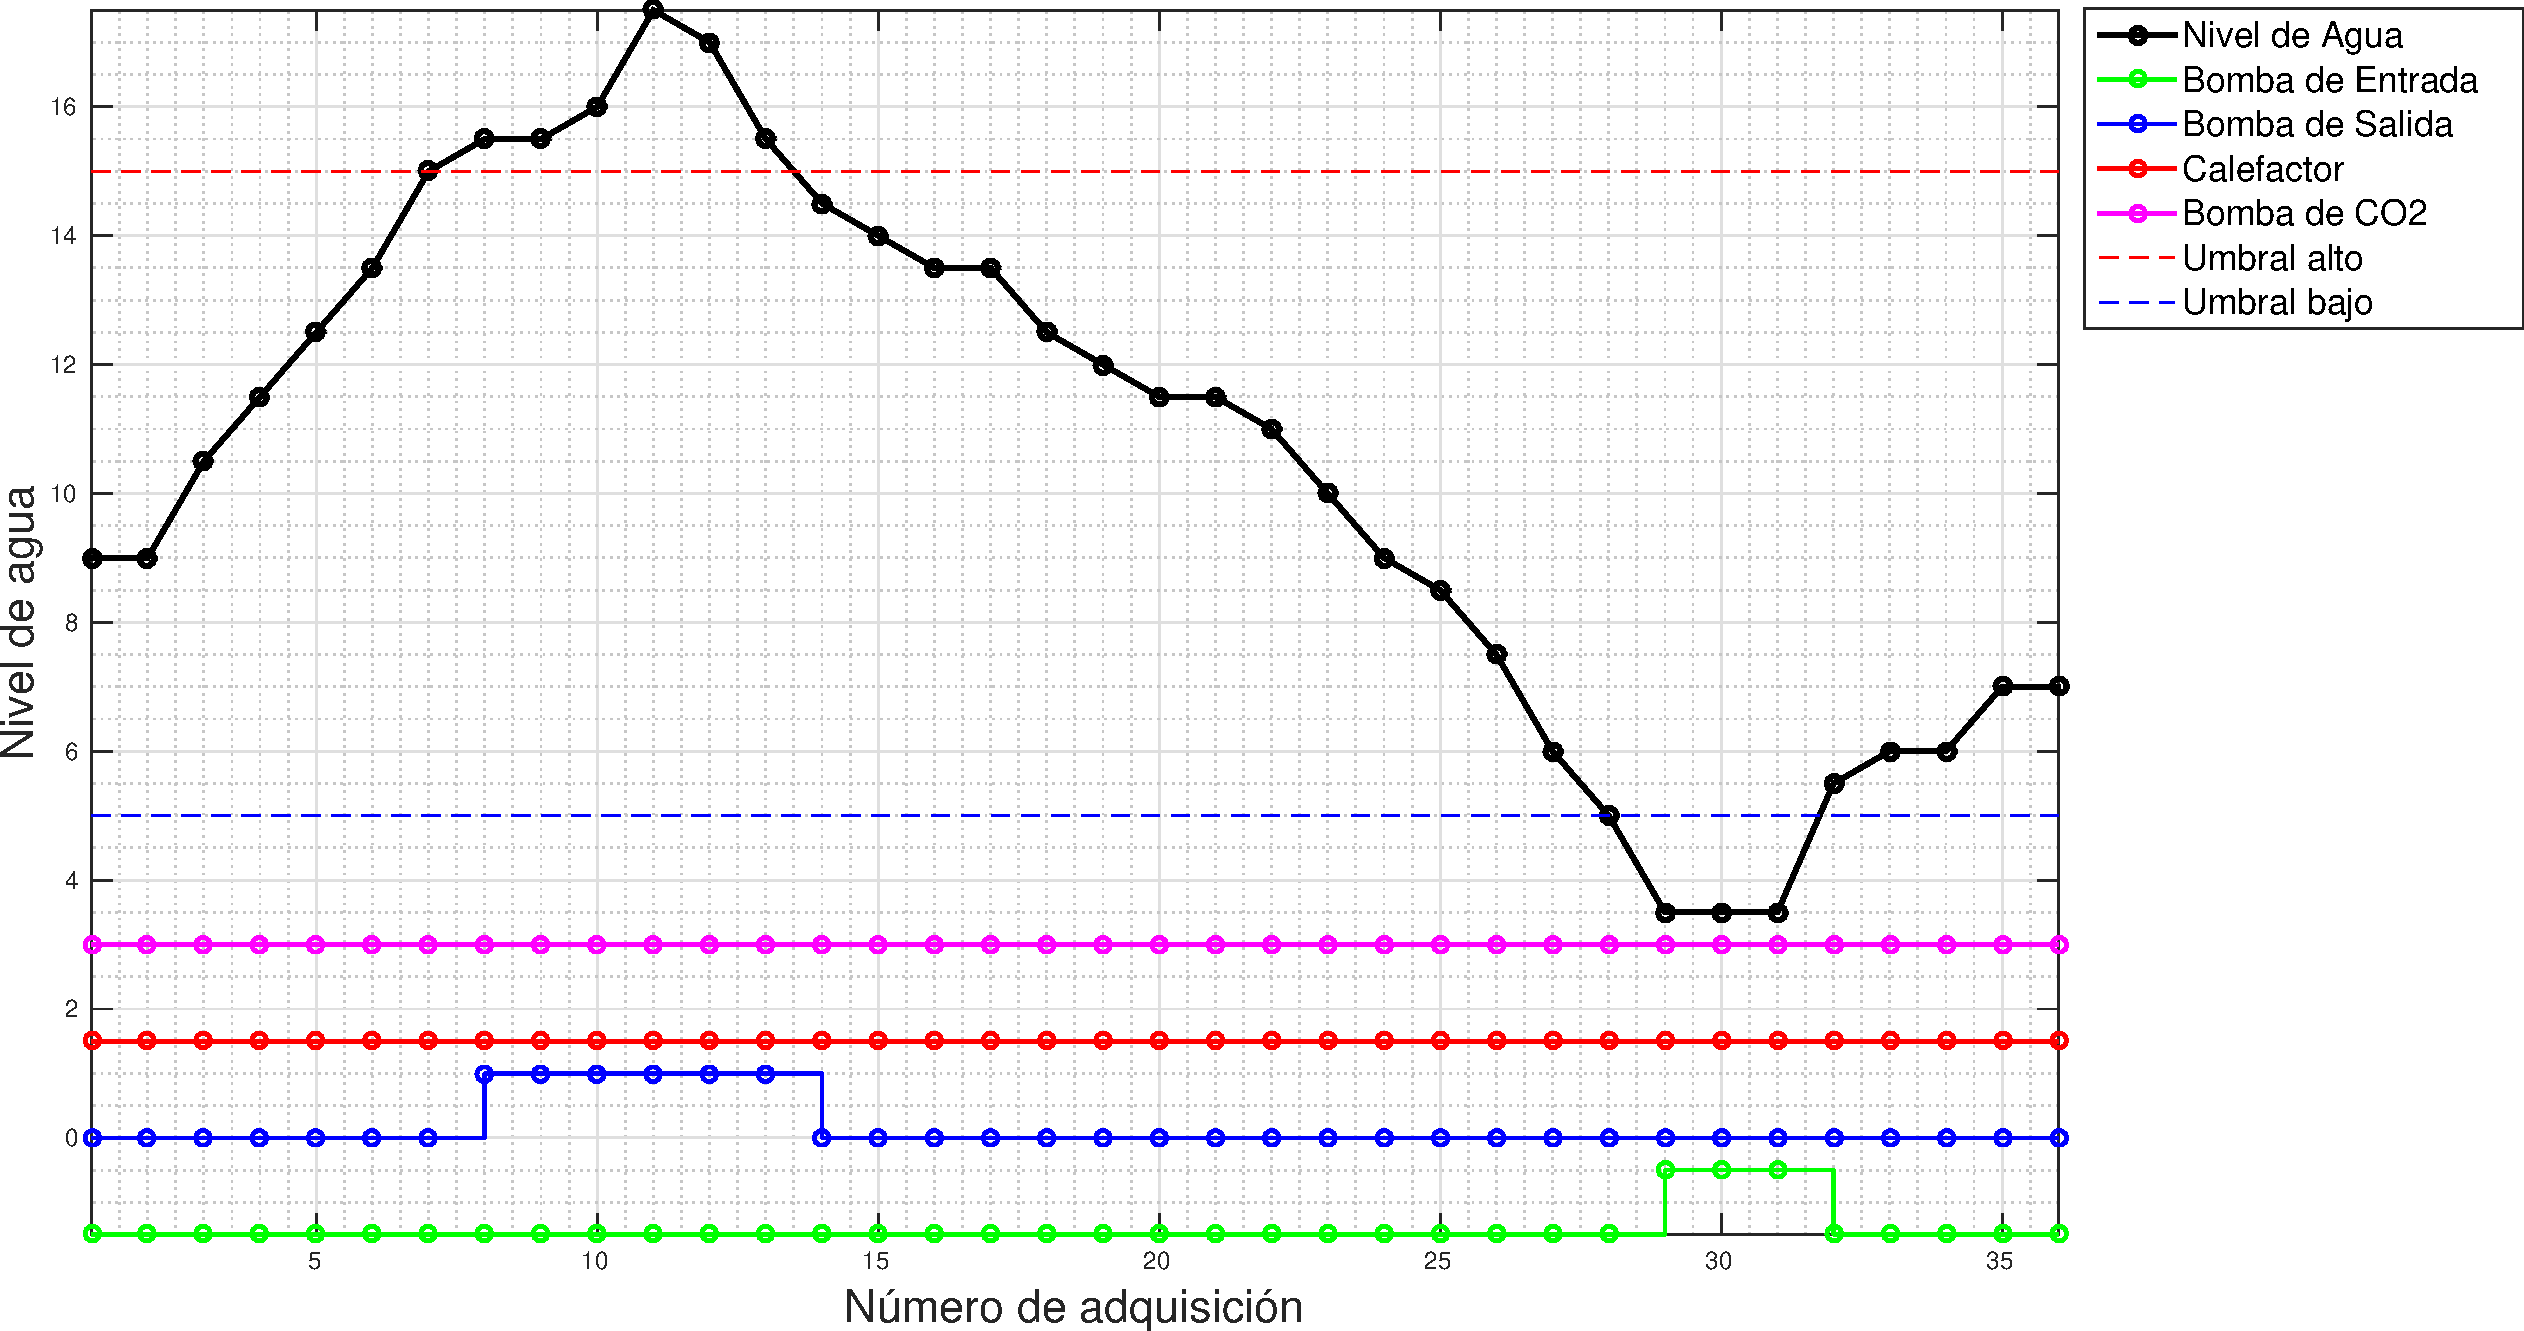
\includegraphics[width=\textwidth]{./Figures/plot1Water.pdf}
	\caption{Respuesta del sistema frente a variaciones en el nivel de agua.}
	\label{fig:alarma1nivel}
\end{figure}

Observando la figura \ref{fig:alarma1nivel}, se puede apreciar que en el momento en que el nivel de agua excede el valor límite superior se enciende la bomba de salida, que luego se apaga cuando valor vuelve a estar en el rango de valores permitidos.  En forma análoga, cuando el nivel de agua supera el valor límite inferior se enciende la bomba de entrada para luego apagarse cuando el valor retorna a niveles normales.

\begin{figure}[h]
\centering
    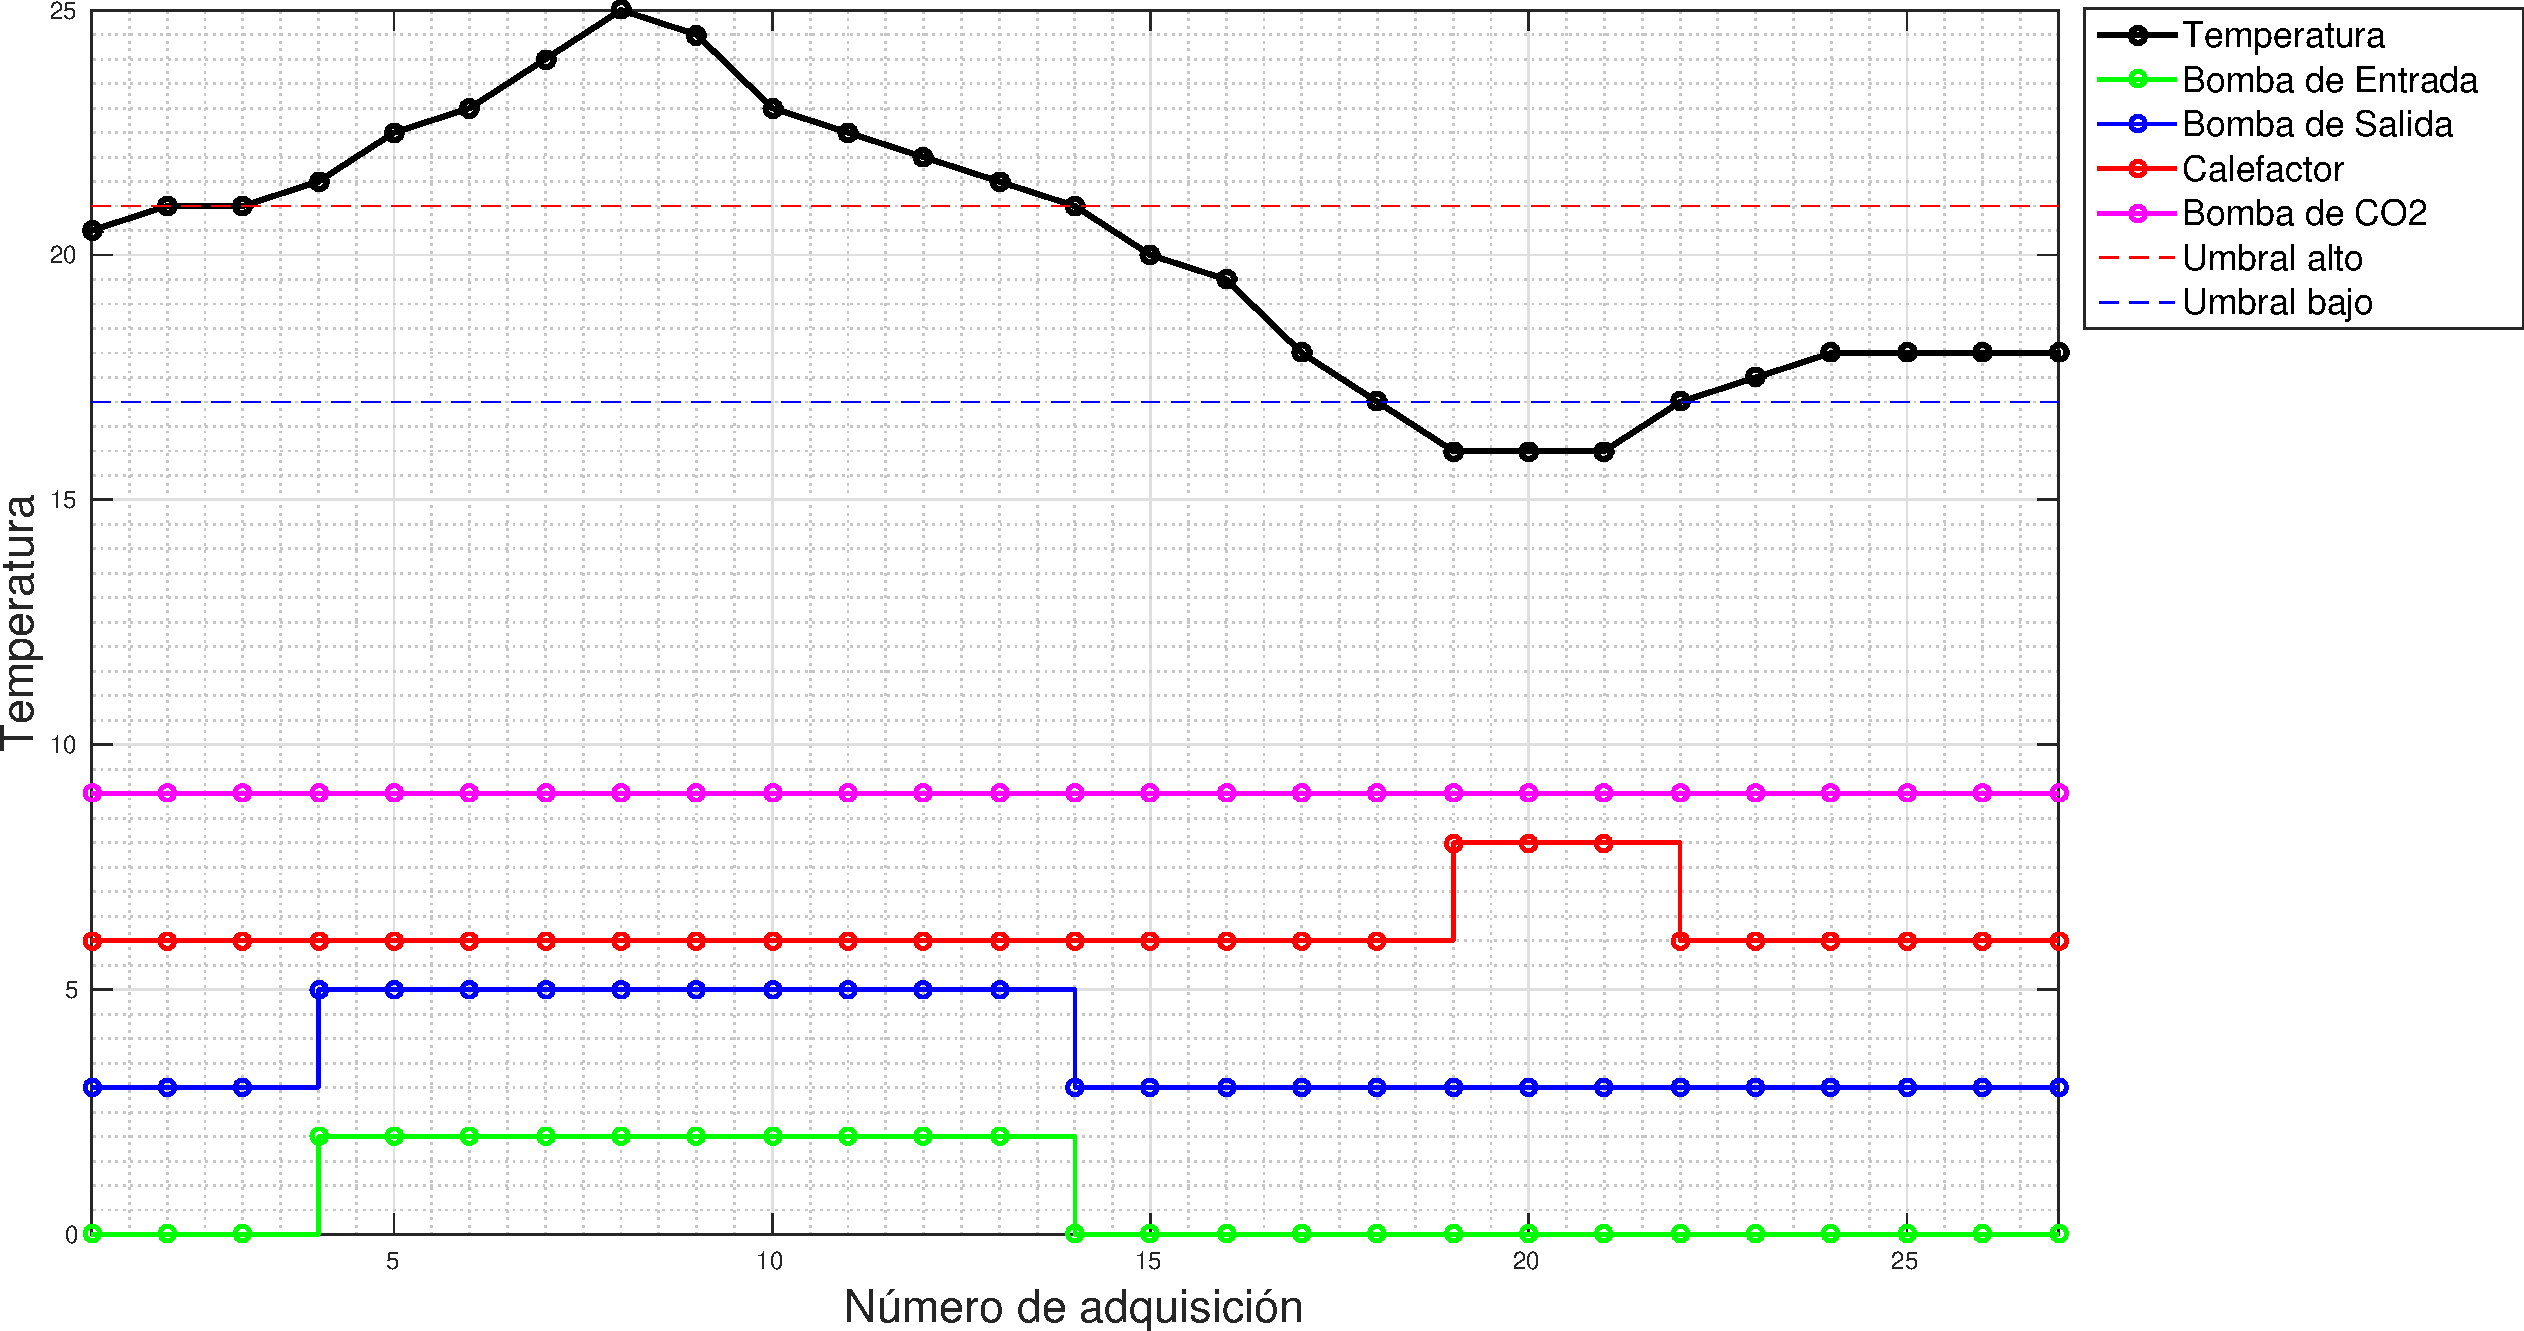
\includegraphics[width=\textwidth]{./Figures/plot1Temp.pdf}
	\caption{Respuesta del sistema frente a variaciones en la temperatura.}
	\label{fig:alarma1Temp}
\end{figure}

Las variaciones en la temperatura en la figura \ref{fig:alarma1Temp} producen que se enciendan las bombas de entrada y salida para recircular el agua cuando el valor excede el límite superior y que se encienda el calefactor cuando el valor de temperatura se encuentra por debajo del límite inferior.  Todas los actuadores que se encienden o apagan por medidas de control vuelven al estado anterior al restablecerse los valores normales de temperatura.

\begin{figure}[h]
\centering
    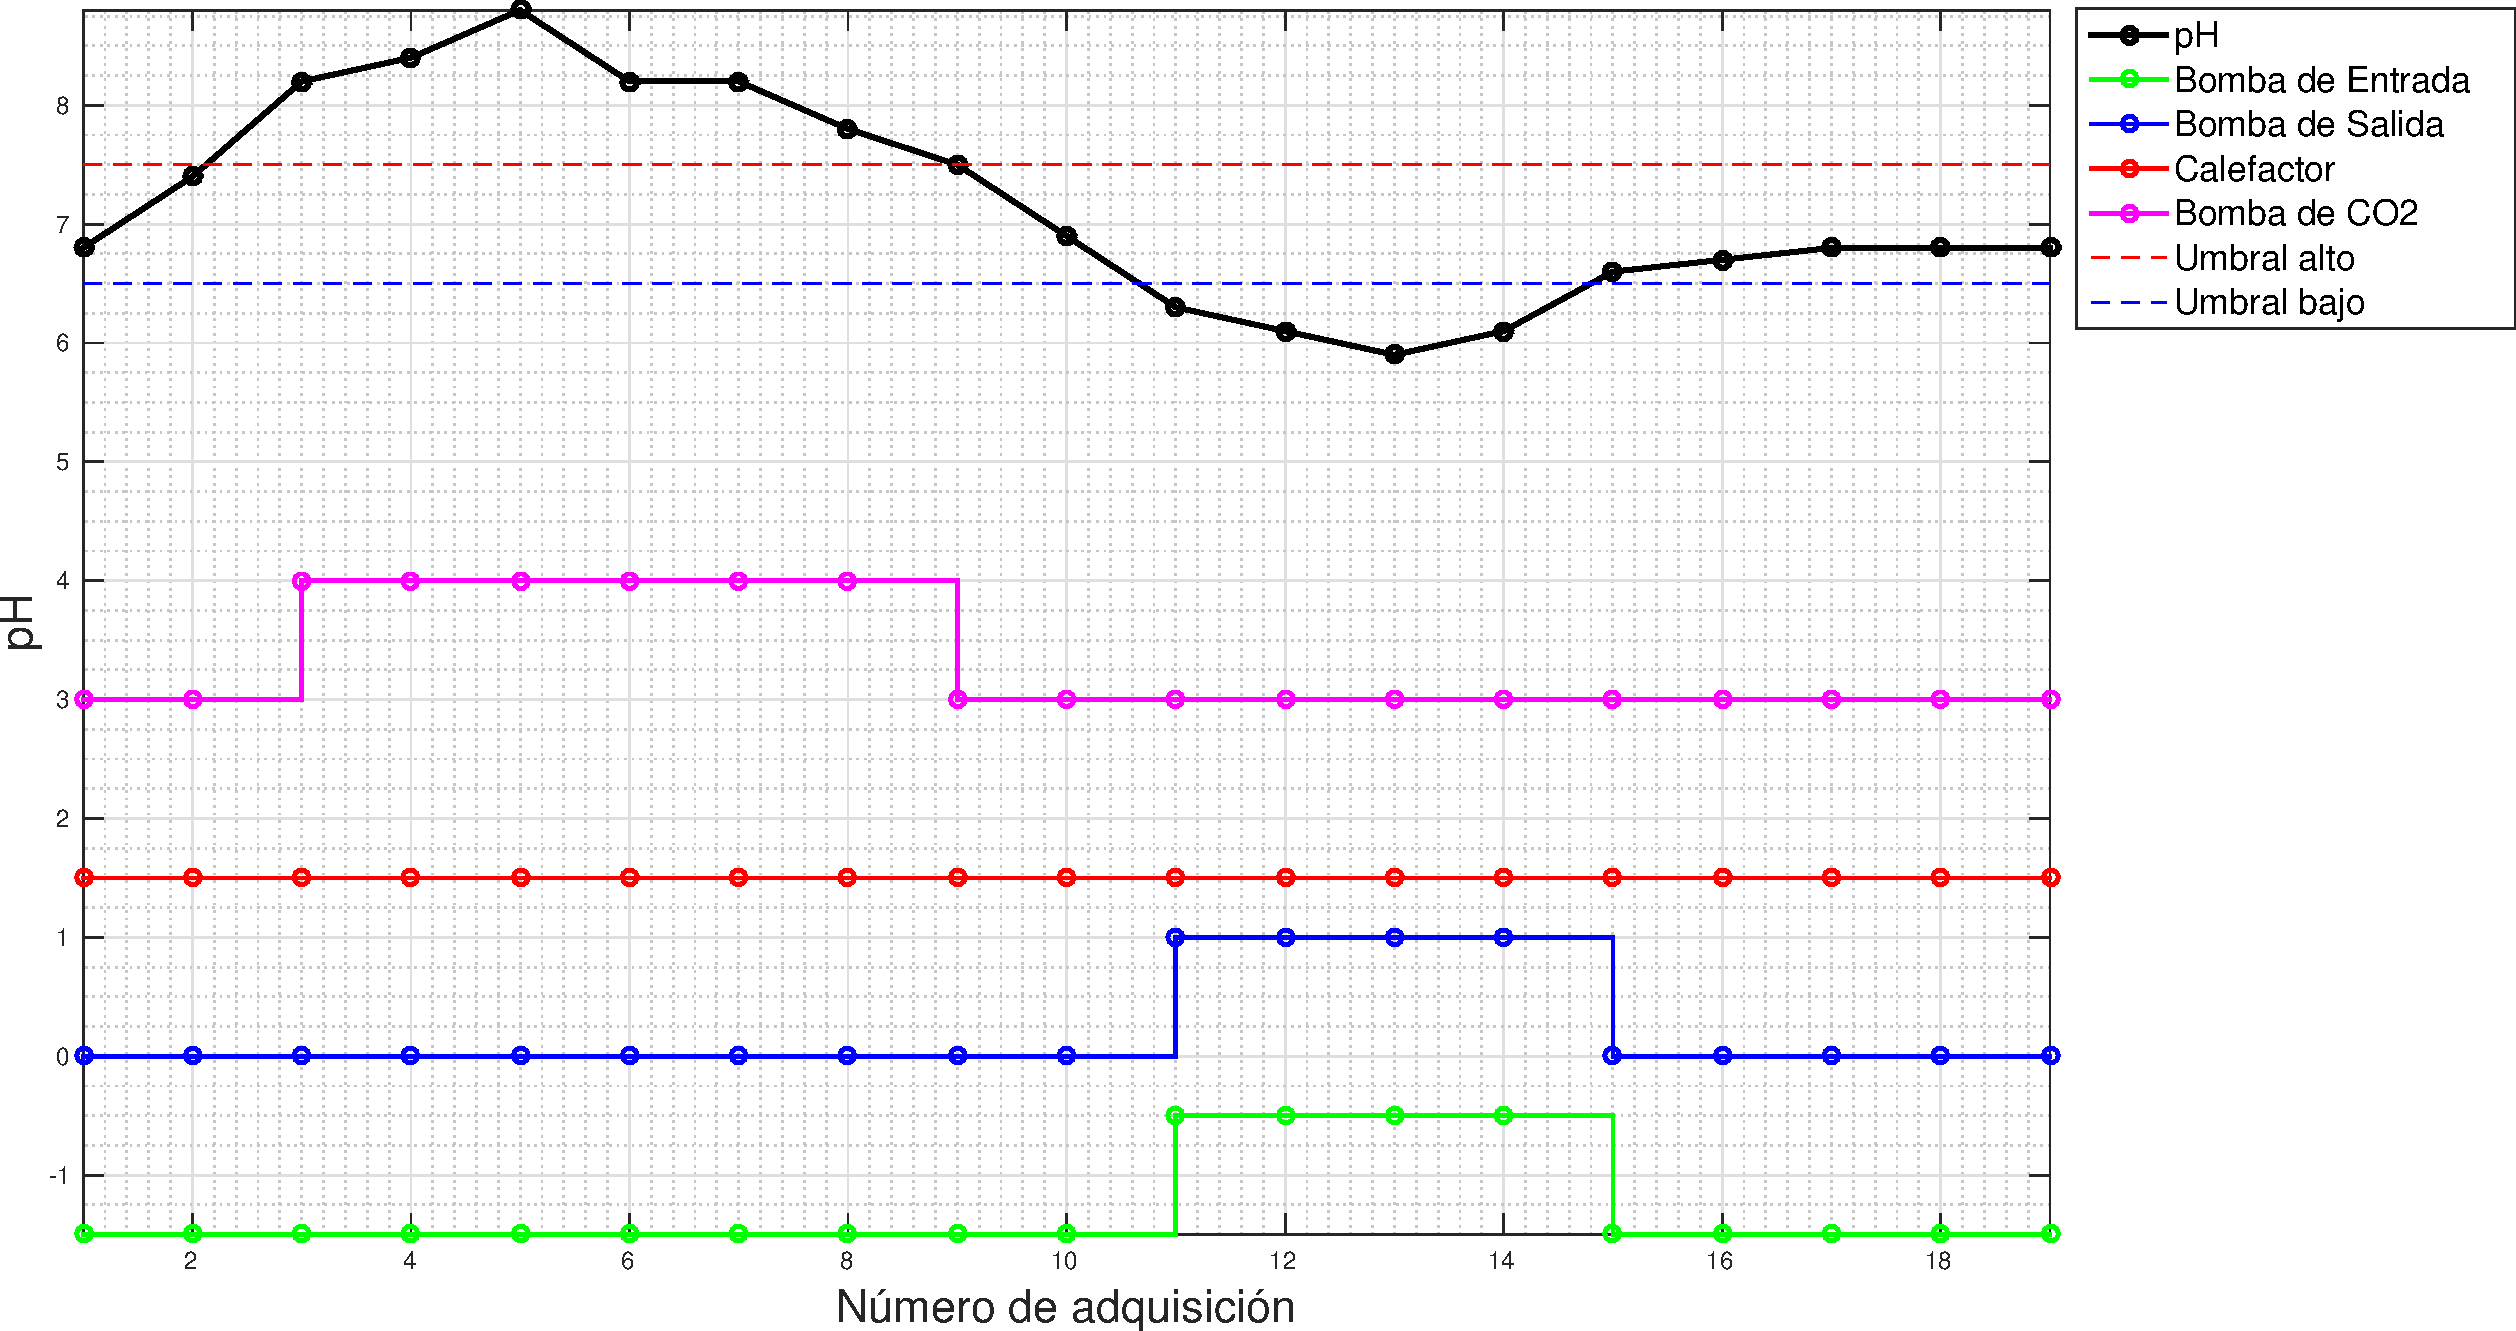
\includegraphics[width=\textwidth]{./Figures/plot1pH.pdf}
	\caption{Respuesta del sistema frente a variaciones en el pH.}
	\label{fig:alarma1pH}
\end{figure}

Como se puede observar en la figura \ref{fig:alarma1pH}, cuando varía el pH se enciende la bomba de $CO_2$ si el valor excede el límite superior, y este actuador se apaga cuando el valor se encuentra por debajo de dicho límite.  En forma similar al comportamiento frente a la alarma de temperatura alta, cuando el valor de pH se encuentra por debajo del límite inferior, se encienden las bombas de entrada y salida para recircular el agua.

\subsection{Respuesta a dos alarmas}
\label{sec:2alarma}

Existen doce combinaciones de dos alarmas al mismo tiempo, según fueron listadas en el cuadro \ref{tab:2alarmas}. En la figura \ref{fig:alarma2WaterHigh} se muestra la respuesta del sistema para las distintas combinaciones de dos alarmas que incluyen la condición de nivel de agua alto.  En la figura \ref{fig:alarma2WaterLow} se puede ver las respuestas frente a las combinaciones de dos alarmas que incluyen la condición de nivel de agua bajo. Finalmente, en la figura \ref{fig:alarma2Temp} se grafica la respuesta frente a las combinaciones de alarma de temperatura alta y baja junto con pH alto y bajo, respectivamente.

A partir de esta sección, los valores límite en línea punteada se grafican del mismo color que el sensor al cual refieren por simplicidad en la visualización.

\begin{figure}[h]
\centering
    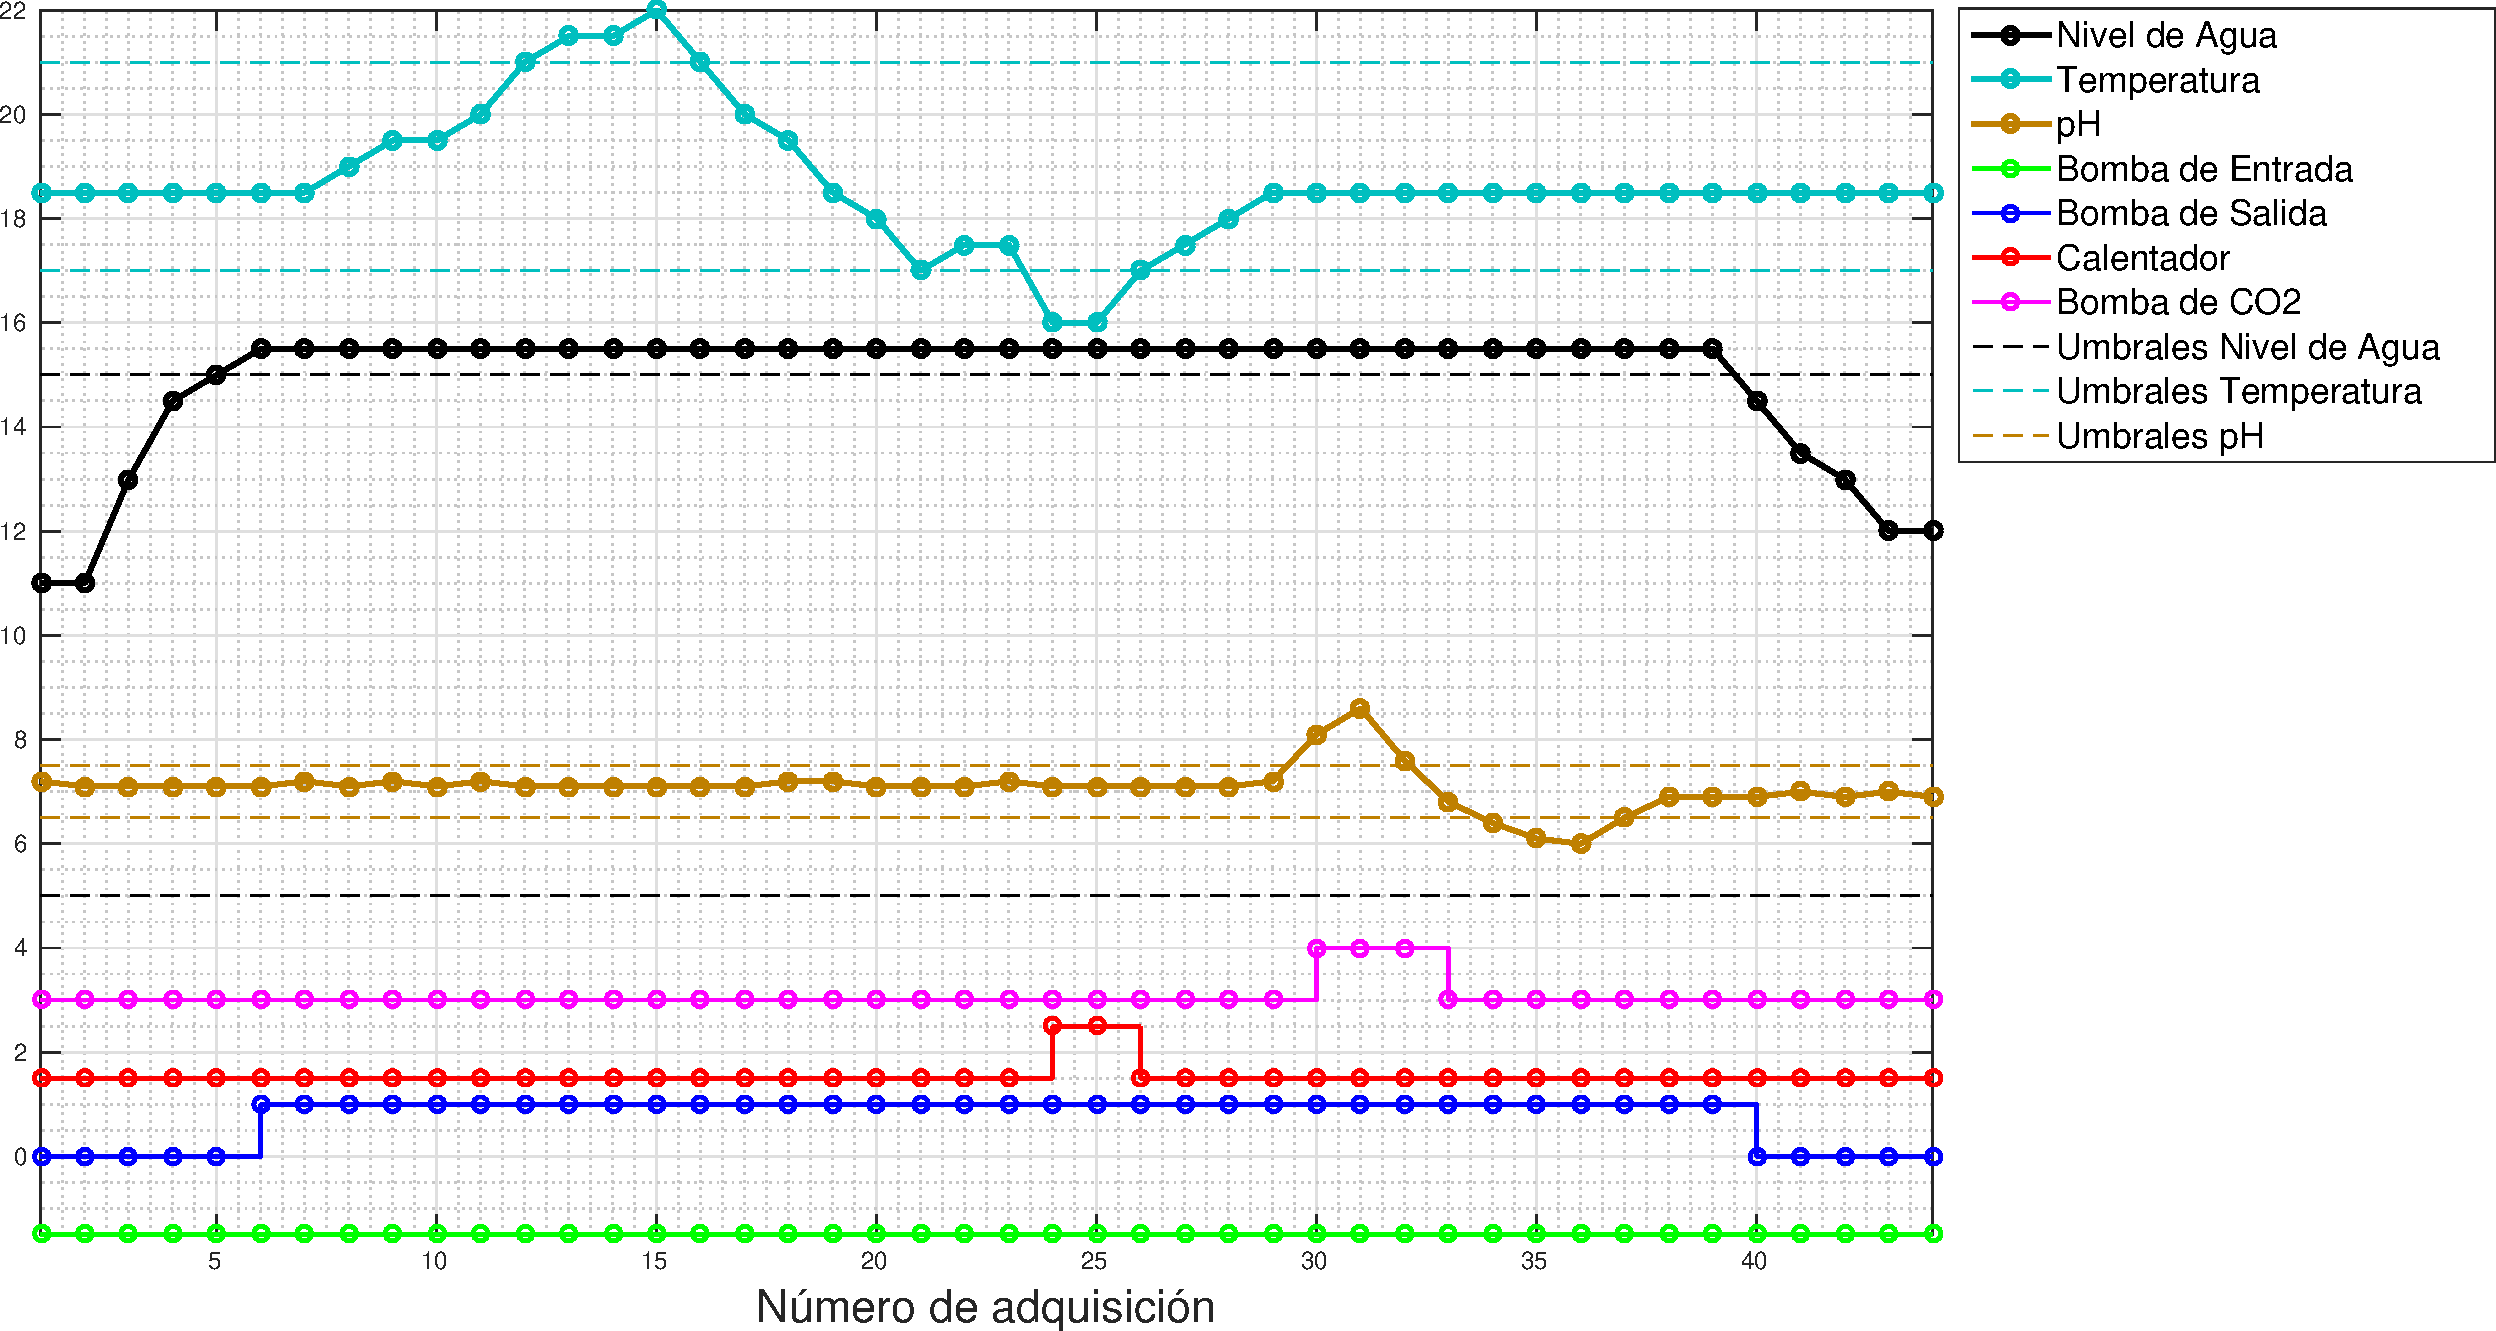
\includegraphics[width=\textwidth]{./Figures/plot2waterHigh.pdf}
	\caption{Respuesta a dos alarmas simultáneas.\\ Nivel de agua alto y otras.}
	\label{fig:alarma2WaterHigh}
\end{figure}

Se puede observar en la figura \ref{fig:alarma2WaterHigh} la condición de nivel de agua alto junto con las de temperatura alta y baja y junto a las de pH alto y bajo posteriormente.  Cabe destacar que cuando la temperatura se encuentra por encima de su valor límite, la bomba de entrada se encuentra inhibida y no se enciende pese a que la acción de contingencia para temperatura alta es ciclar el agua.  Esto se debe a que la condición de nivel de agua alto tiene mayor prioridad.  Lo mismo ocurre con la condición de pH bajo que tiene la misma acción de contingencia que la de temperatura alta. Durante todo el tiempo que el nivel de agua supera su valor límite, la bomba de salida se encuentra encendida.

De manera análoga al análisis precedente, en la figura \ref{fig:alarma2WaterLow} se muestran condiciones de dos alarmas simultáneas donde una de ellas es la de nivel de agua bajo. En este caso, frente a las condiciones de temperatura alta y pH bajo, el actuador que se encuentra inhibido es la bomba de salida porque la condición de nivel de agua bajo tiene mayor prioridad que las anteriores. Durante todo el tiempo que el nivel de agua se encuentra por debajo de su límite inferior, la bomba de entrada permanece encendida y se apaga cuando el nivel de agua vuelve a estar entre los valores permitidos.

\vspace{20px}
\begin{figure}[htpb!]
\centering
    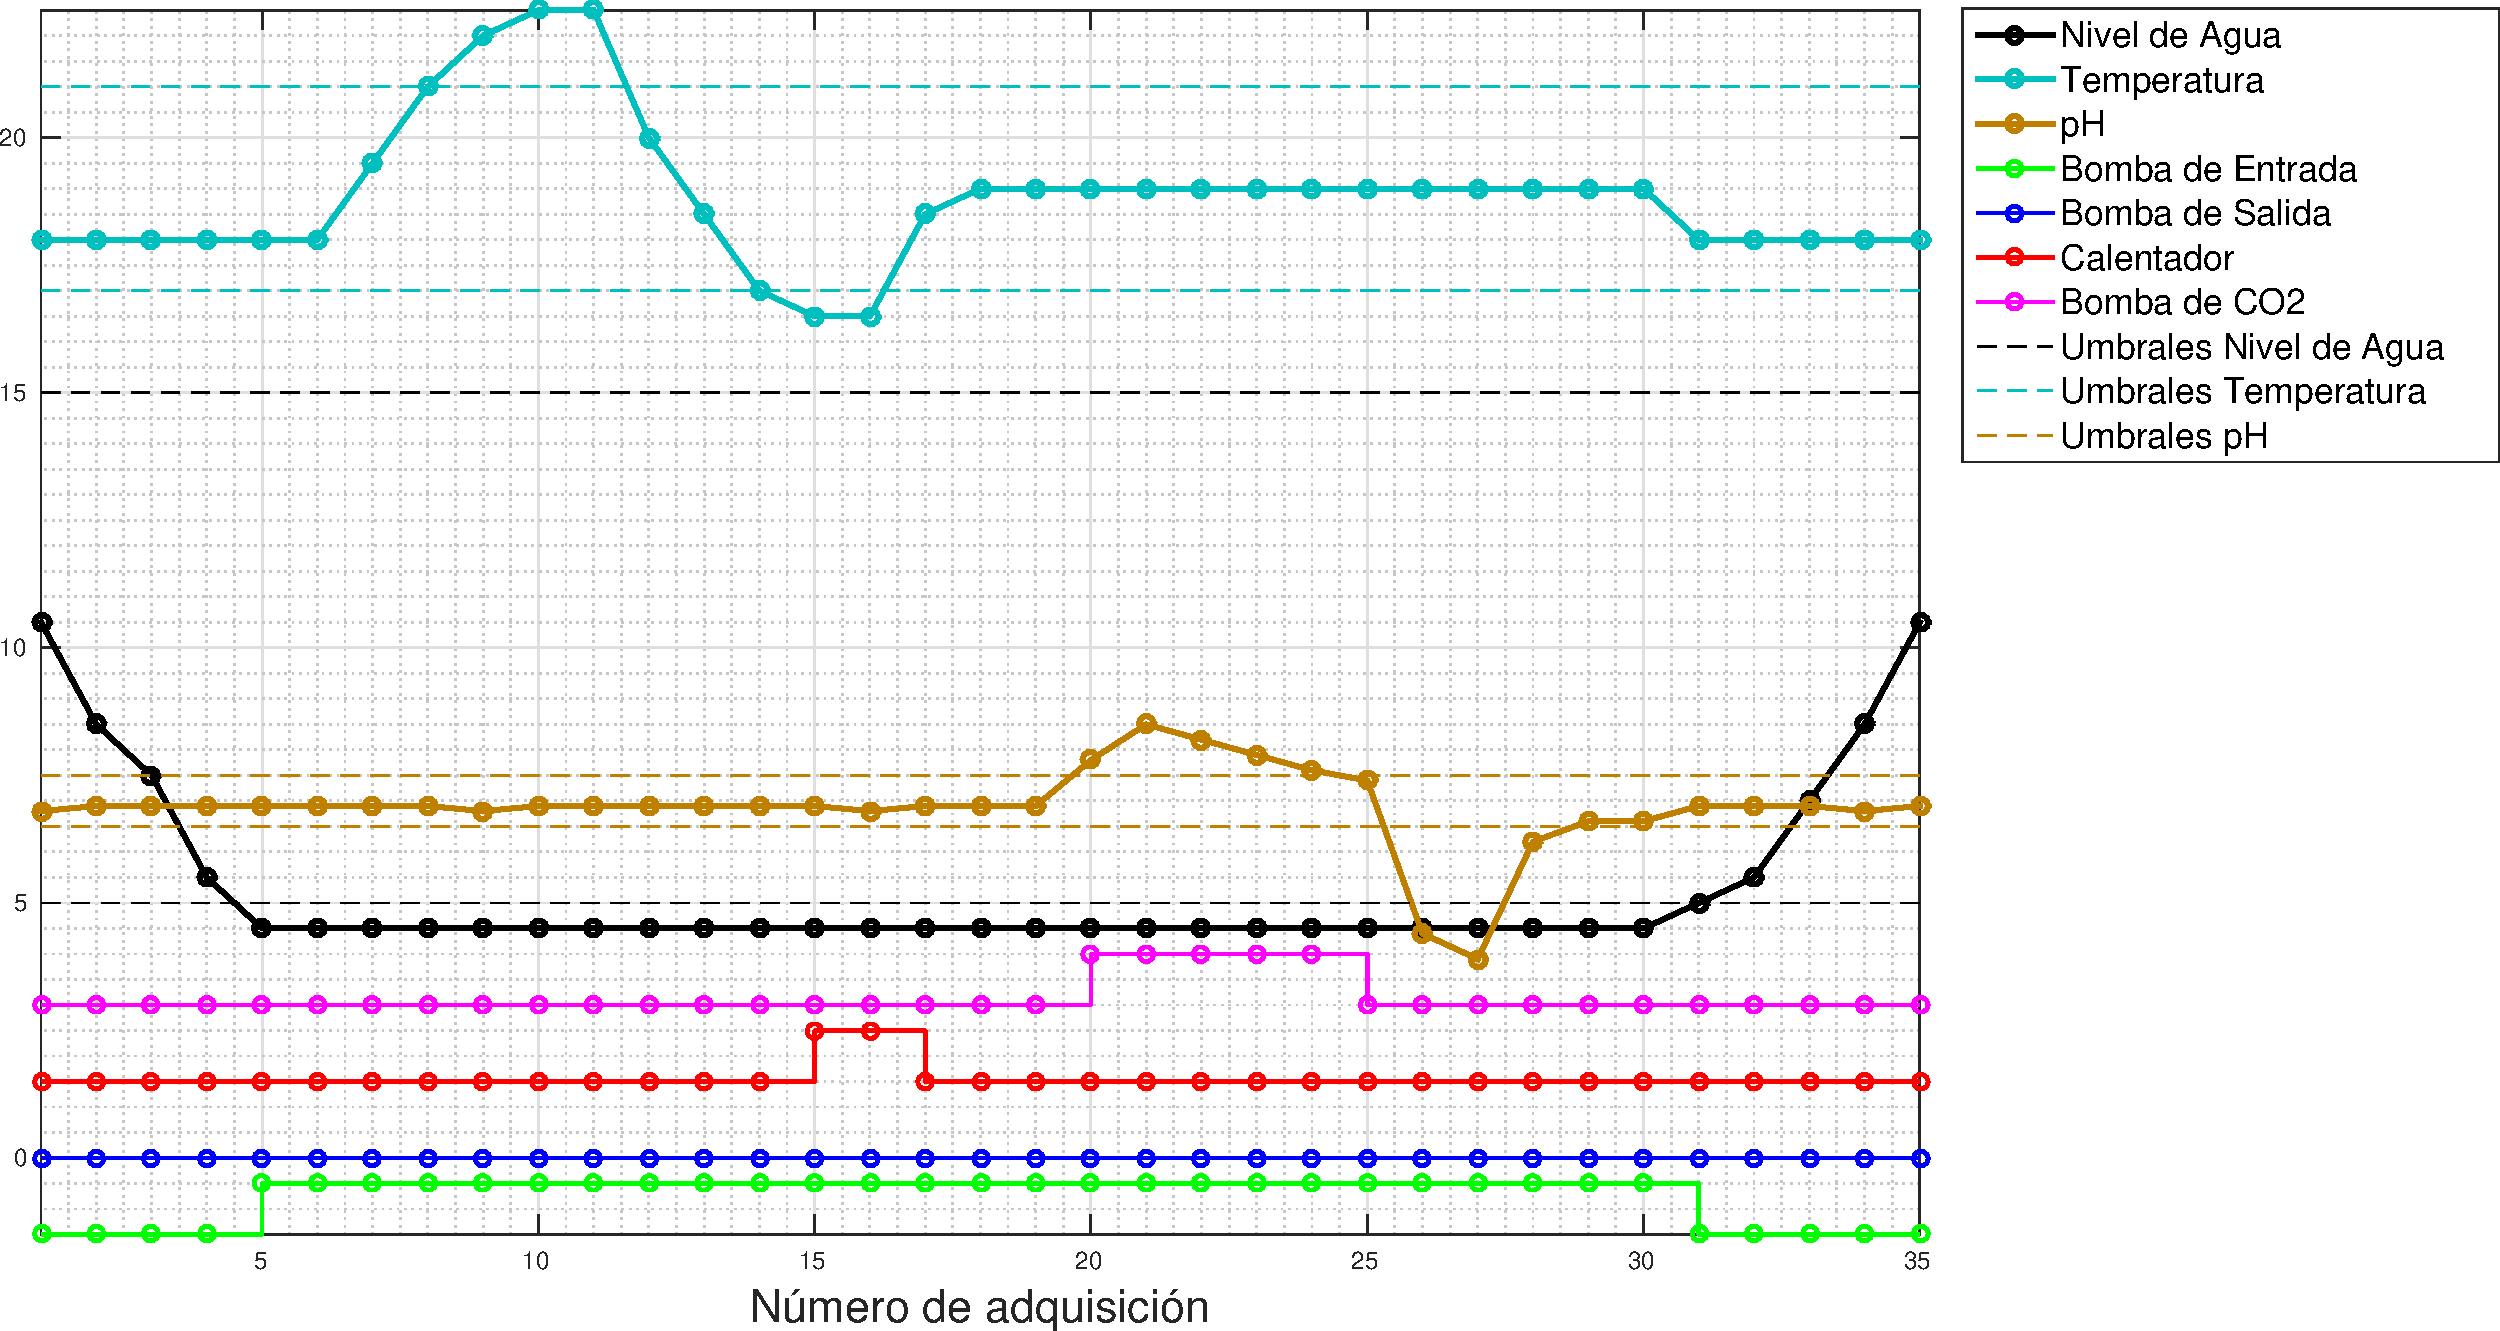
\includegraphics[width=\textwidth]{./Figures/plot2waterLow.pdf}
	\caption{Respuesta a dos alarmas simultáneas.\\ Nivel de agua bajo y otras.}
	\label{fig:alarma2WaterLow}
\end{figure}

Las últimas cuatro combinaciones de dos alarmas se producen entre las asociadas a los sensores de temperatura y pH.  En la figura \ref{fig:alarma2Temp} se puede observar cómo se encienden las bombas de entrada y salida si al menos una de las condiciones de temperatura alta o pH bajo están presentes.  Por otra parte, si la temperatura se encuentra por debajo de su valor mínimo permitido se enciende el calefactor y si el pH supera su límite se enciende la bomba de $CO_2$.

\vspace{20px}

\begin{figure}[htpb!]
\centering
    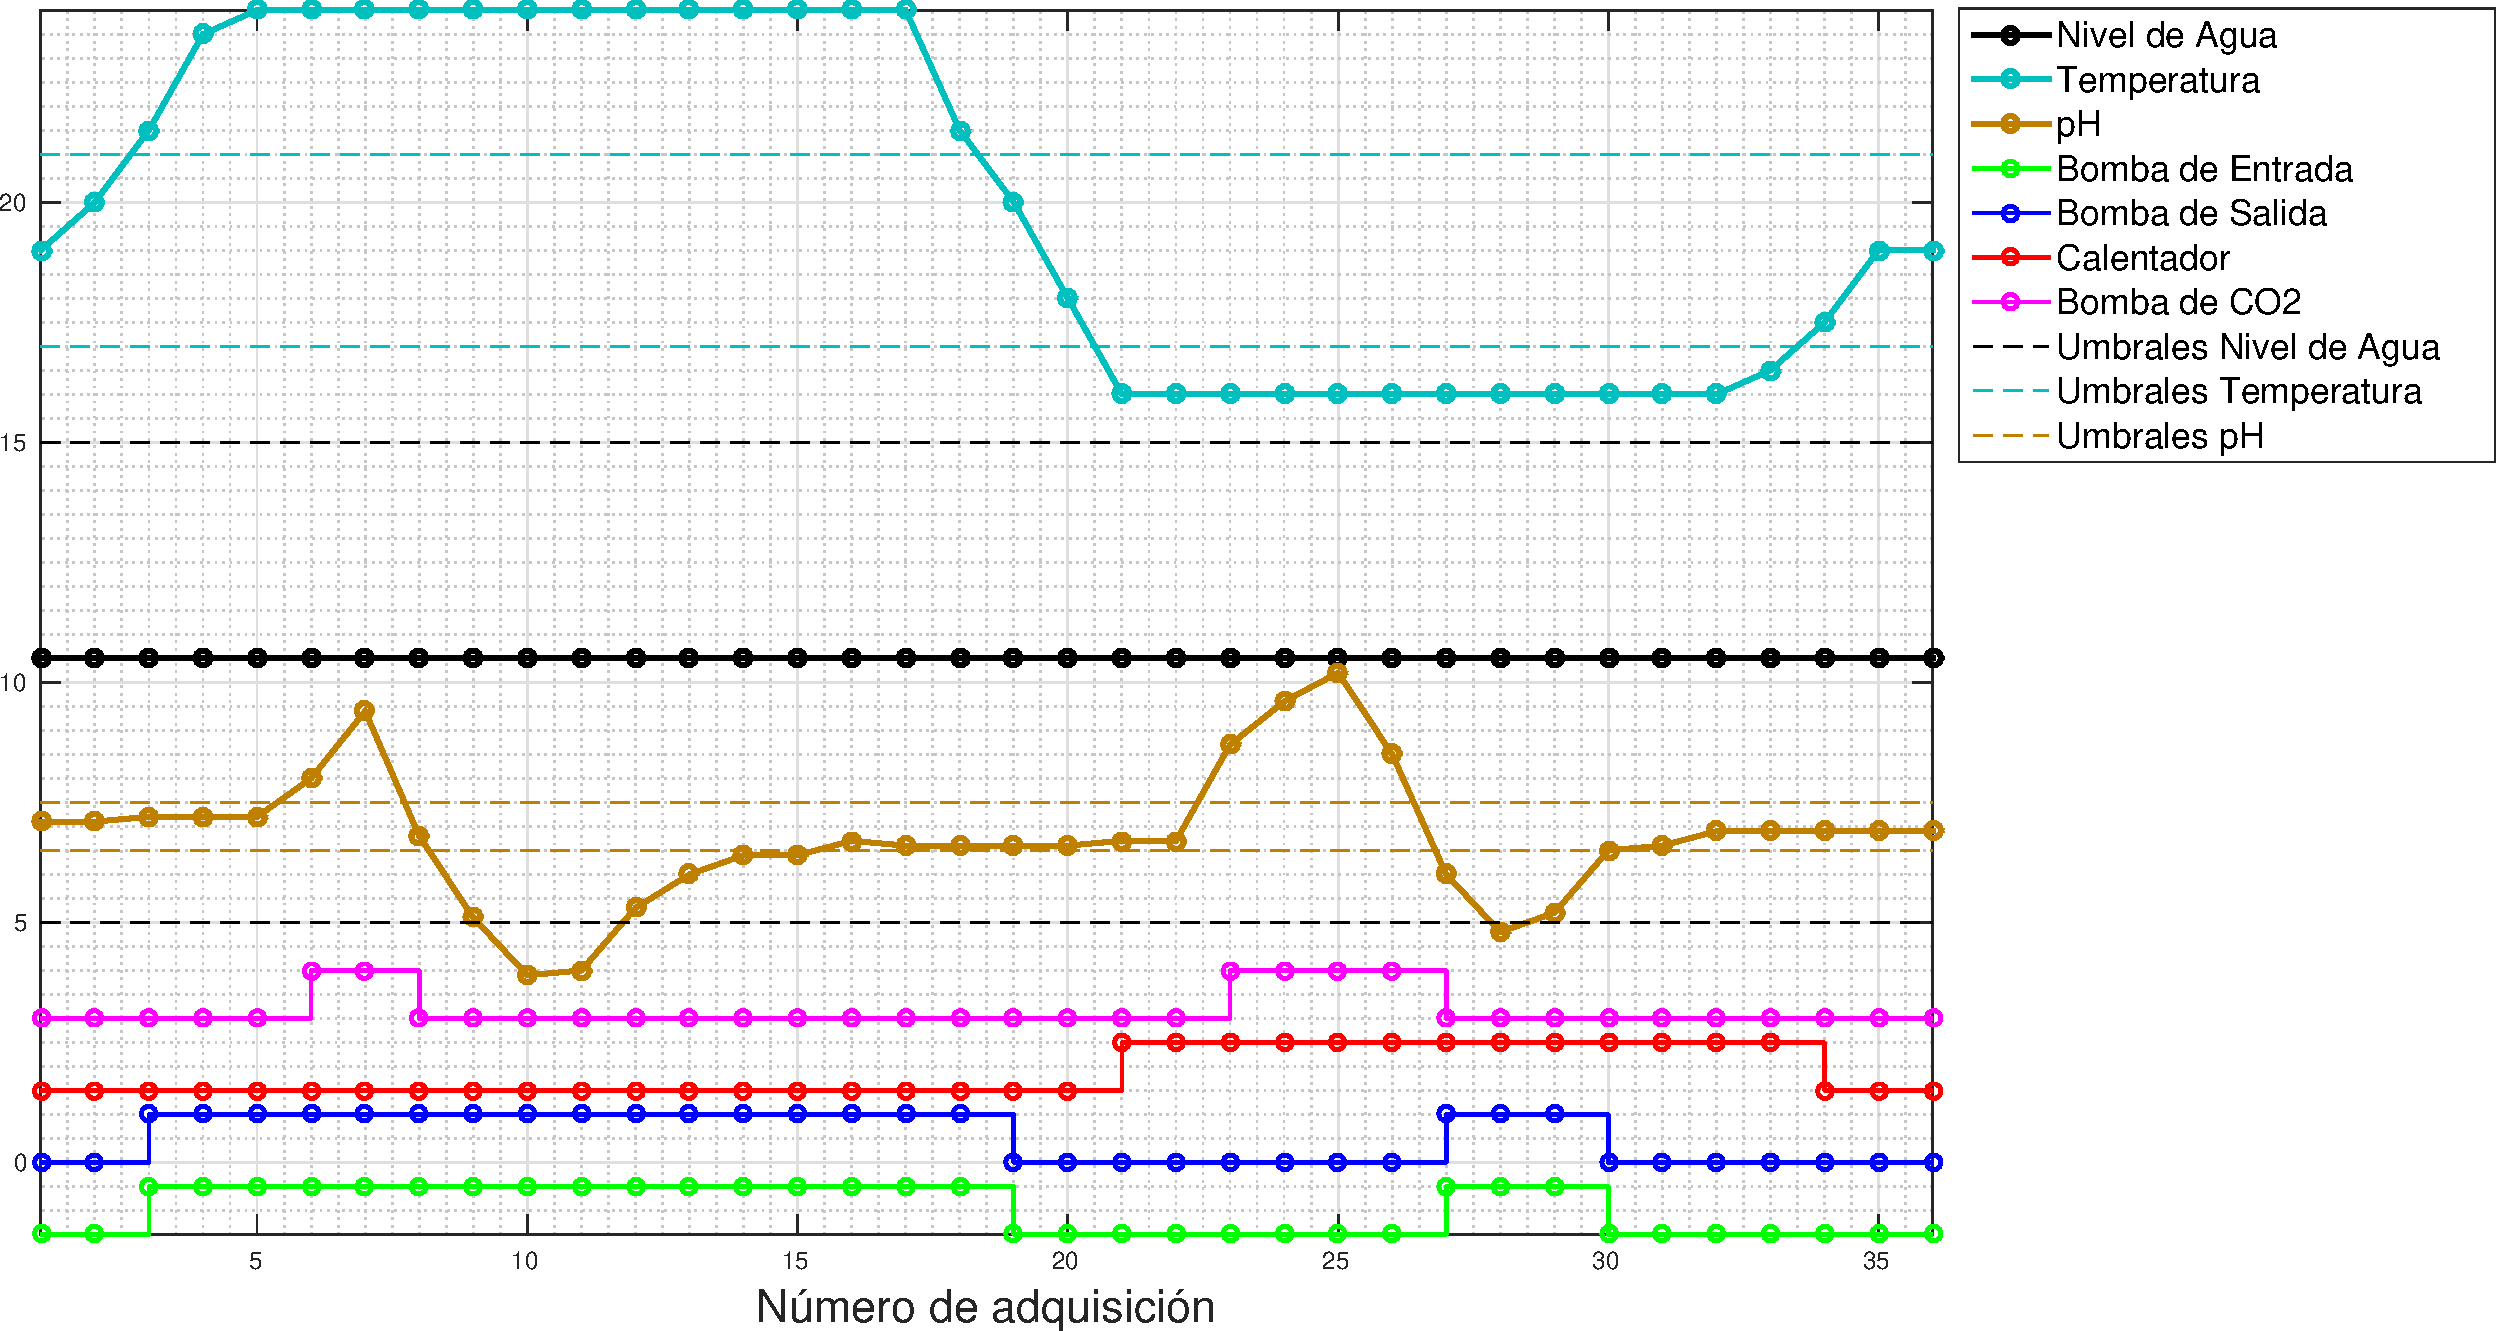
\includegraphics[width=\textwidth]{./Figures/plot2Temp.pdf}
	\caption{Respuesta a dos alarmas simultáneas.\\ Temperatura y pH.}
	\label{fig:alarma2Temp}
\end{figure}

\clearpage
\subsection{Respuesta a tres alarmas}
\label{sec:3alarma}

Existen 8 combinaciones de 3 alarmas simultáneas según fueron listadas en el cuadro \ref{tab:3alarmas}. Se presentan agrupadas en dos gráficas, en las figuras \ref{fig:alarma3WaterHigh} y \ref{fig:alarma3WaterLow}, según se mantenga fija la condición de alarma por nivel de agua alto o bajo, respectivamente.

Se puede observar en la figura \ref{fig:alarma3WaterHigh}, que las acciones de control de alarma son las esperadas, teniendo en cuenta que, al igual que en el caso de dos alarmas, cuando se encuentra presente la condición de alarma de nivel de agua alto, se inhibe el encendido de la bomba de entrada.

\begin{figure}[hp]
\centering
    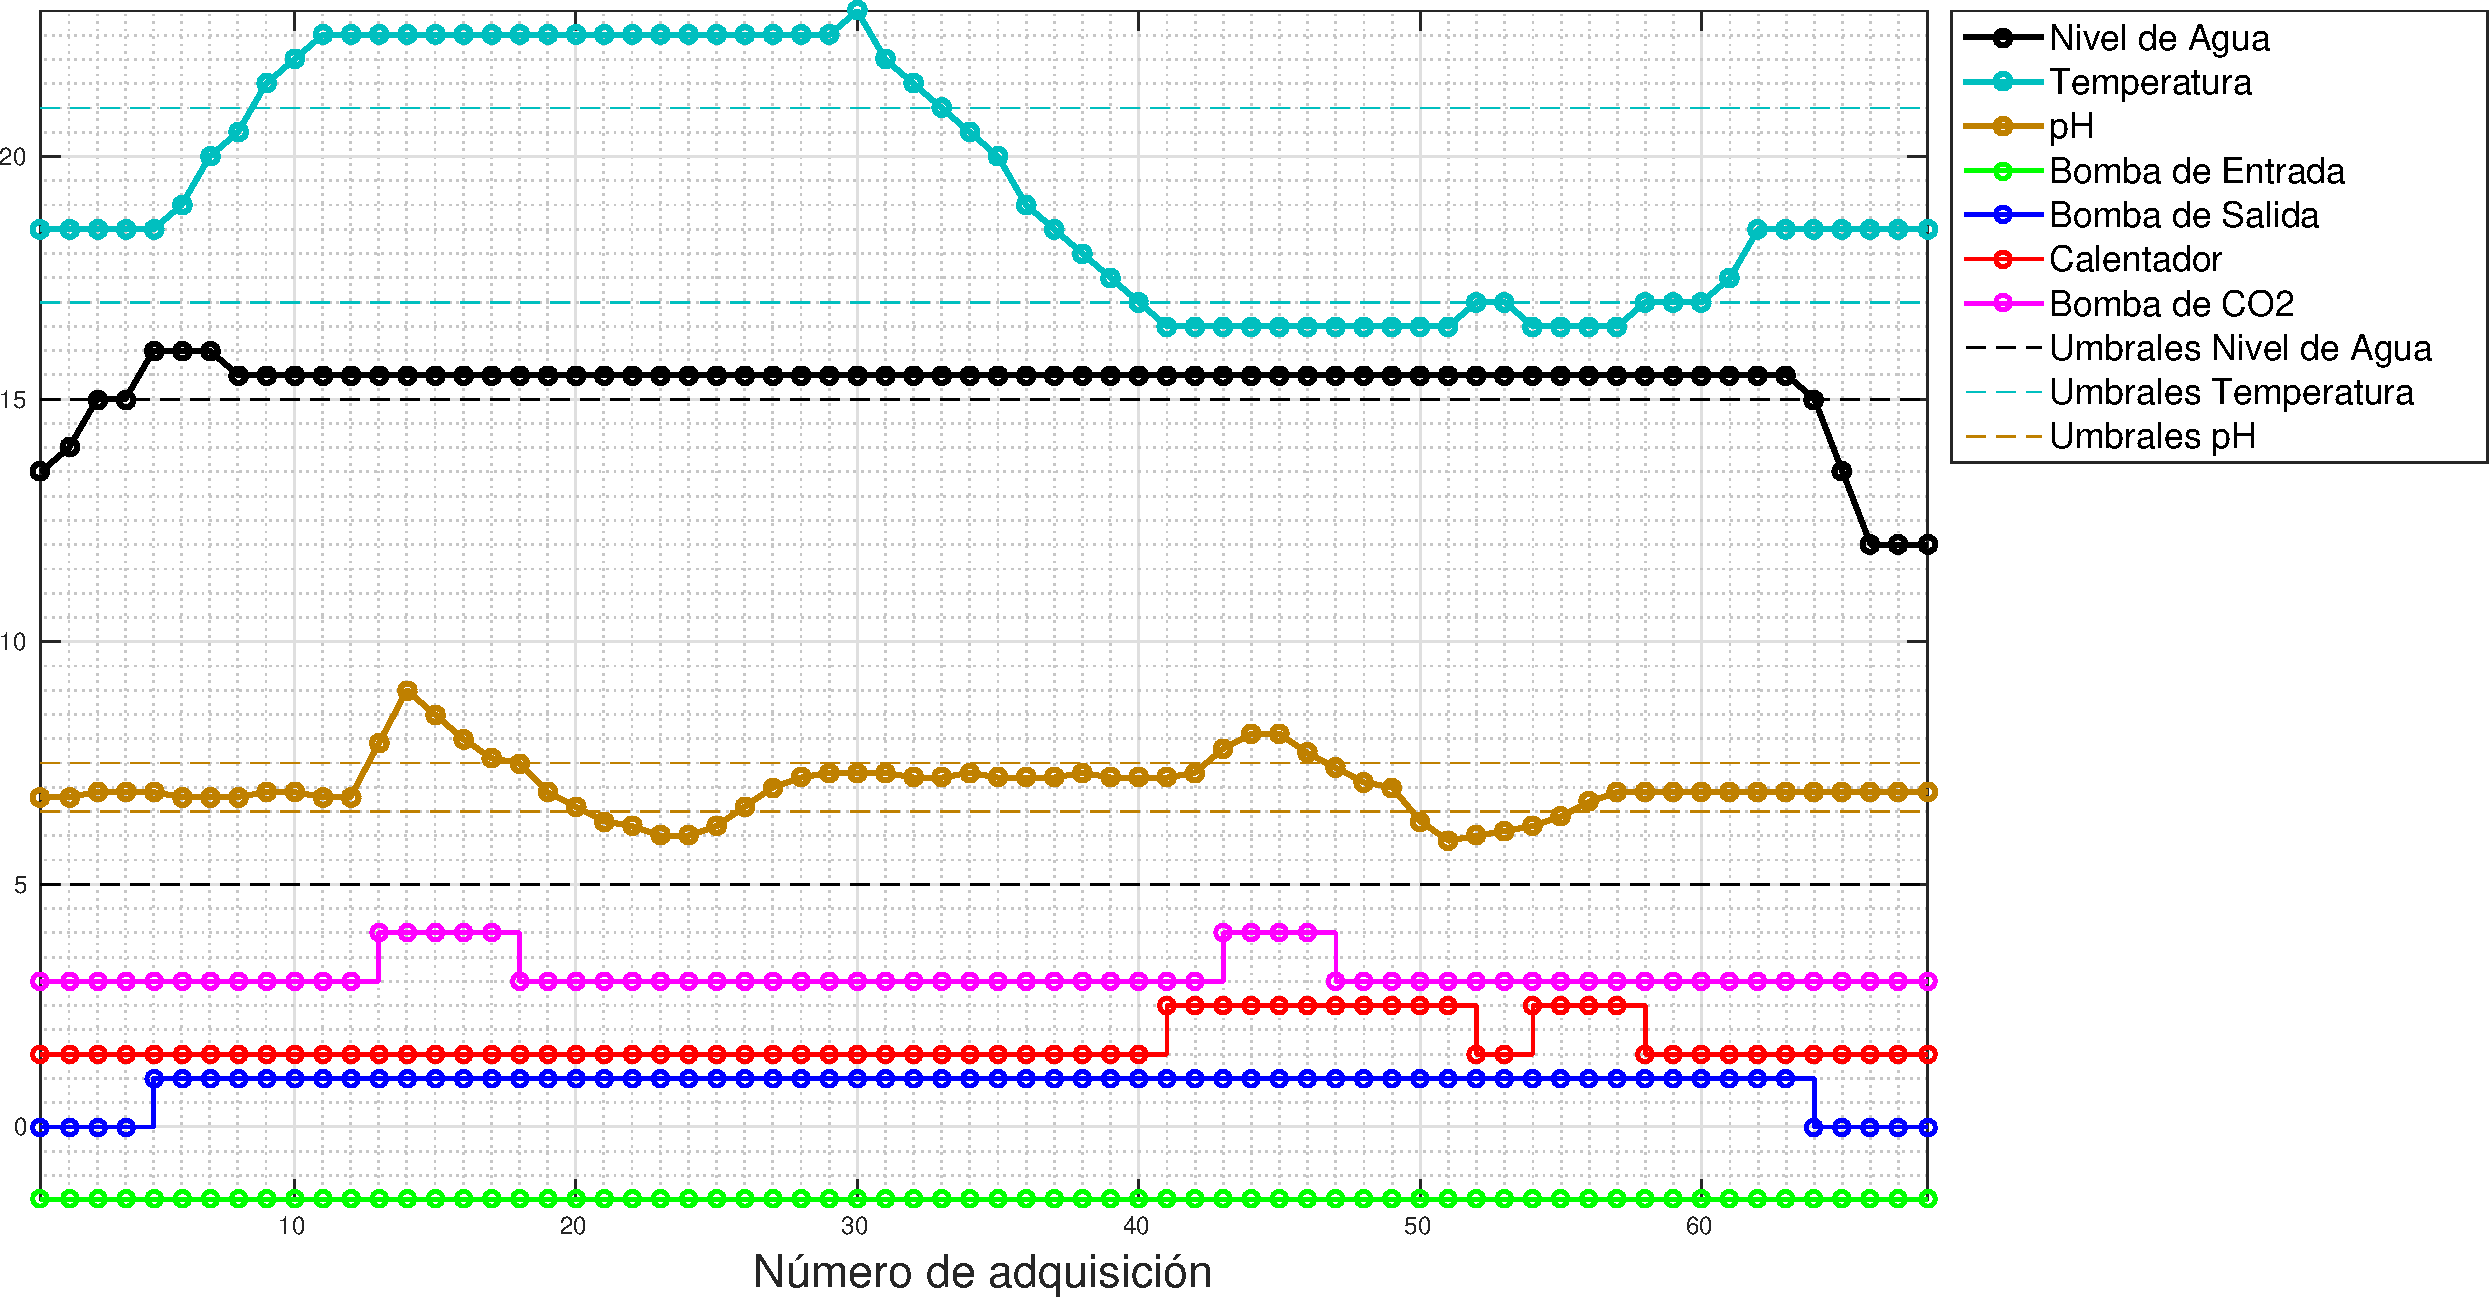
\includegraphics[width=\textwidth]{./Figures/plot3waterHigh.pdf}
	\caption[Respuesta a tres alarmas simultáneas. Nivel de agua alto y otras.]{Tres alarmas: nivel de agua alto y otras.}
	\label{fig:alarma3WaterHigh}
\end{figure}

En forma análoga al análisis precedente, en la figura \ref{fig:alarma3WaterLow} se puede observar que las acciones de control son las esperadas, teniendo en cuenta que en este caso el actuador inhibido es la bomba de salida por la condición de alarma de nivel de agua bajo.

\begin{figure}[hp]
\centering
    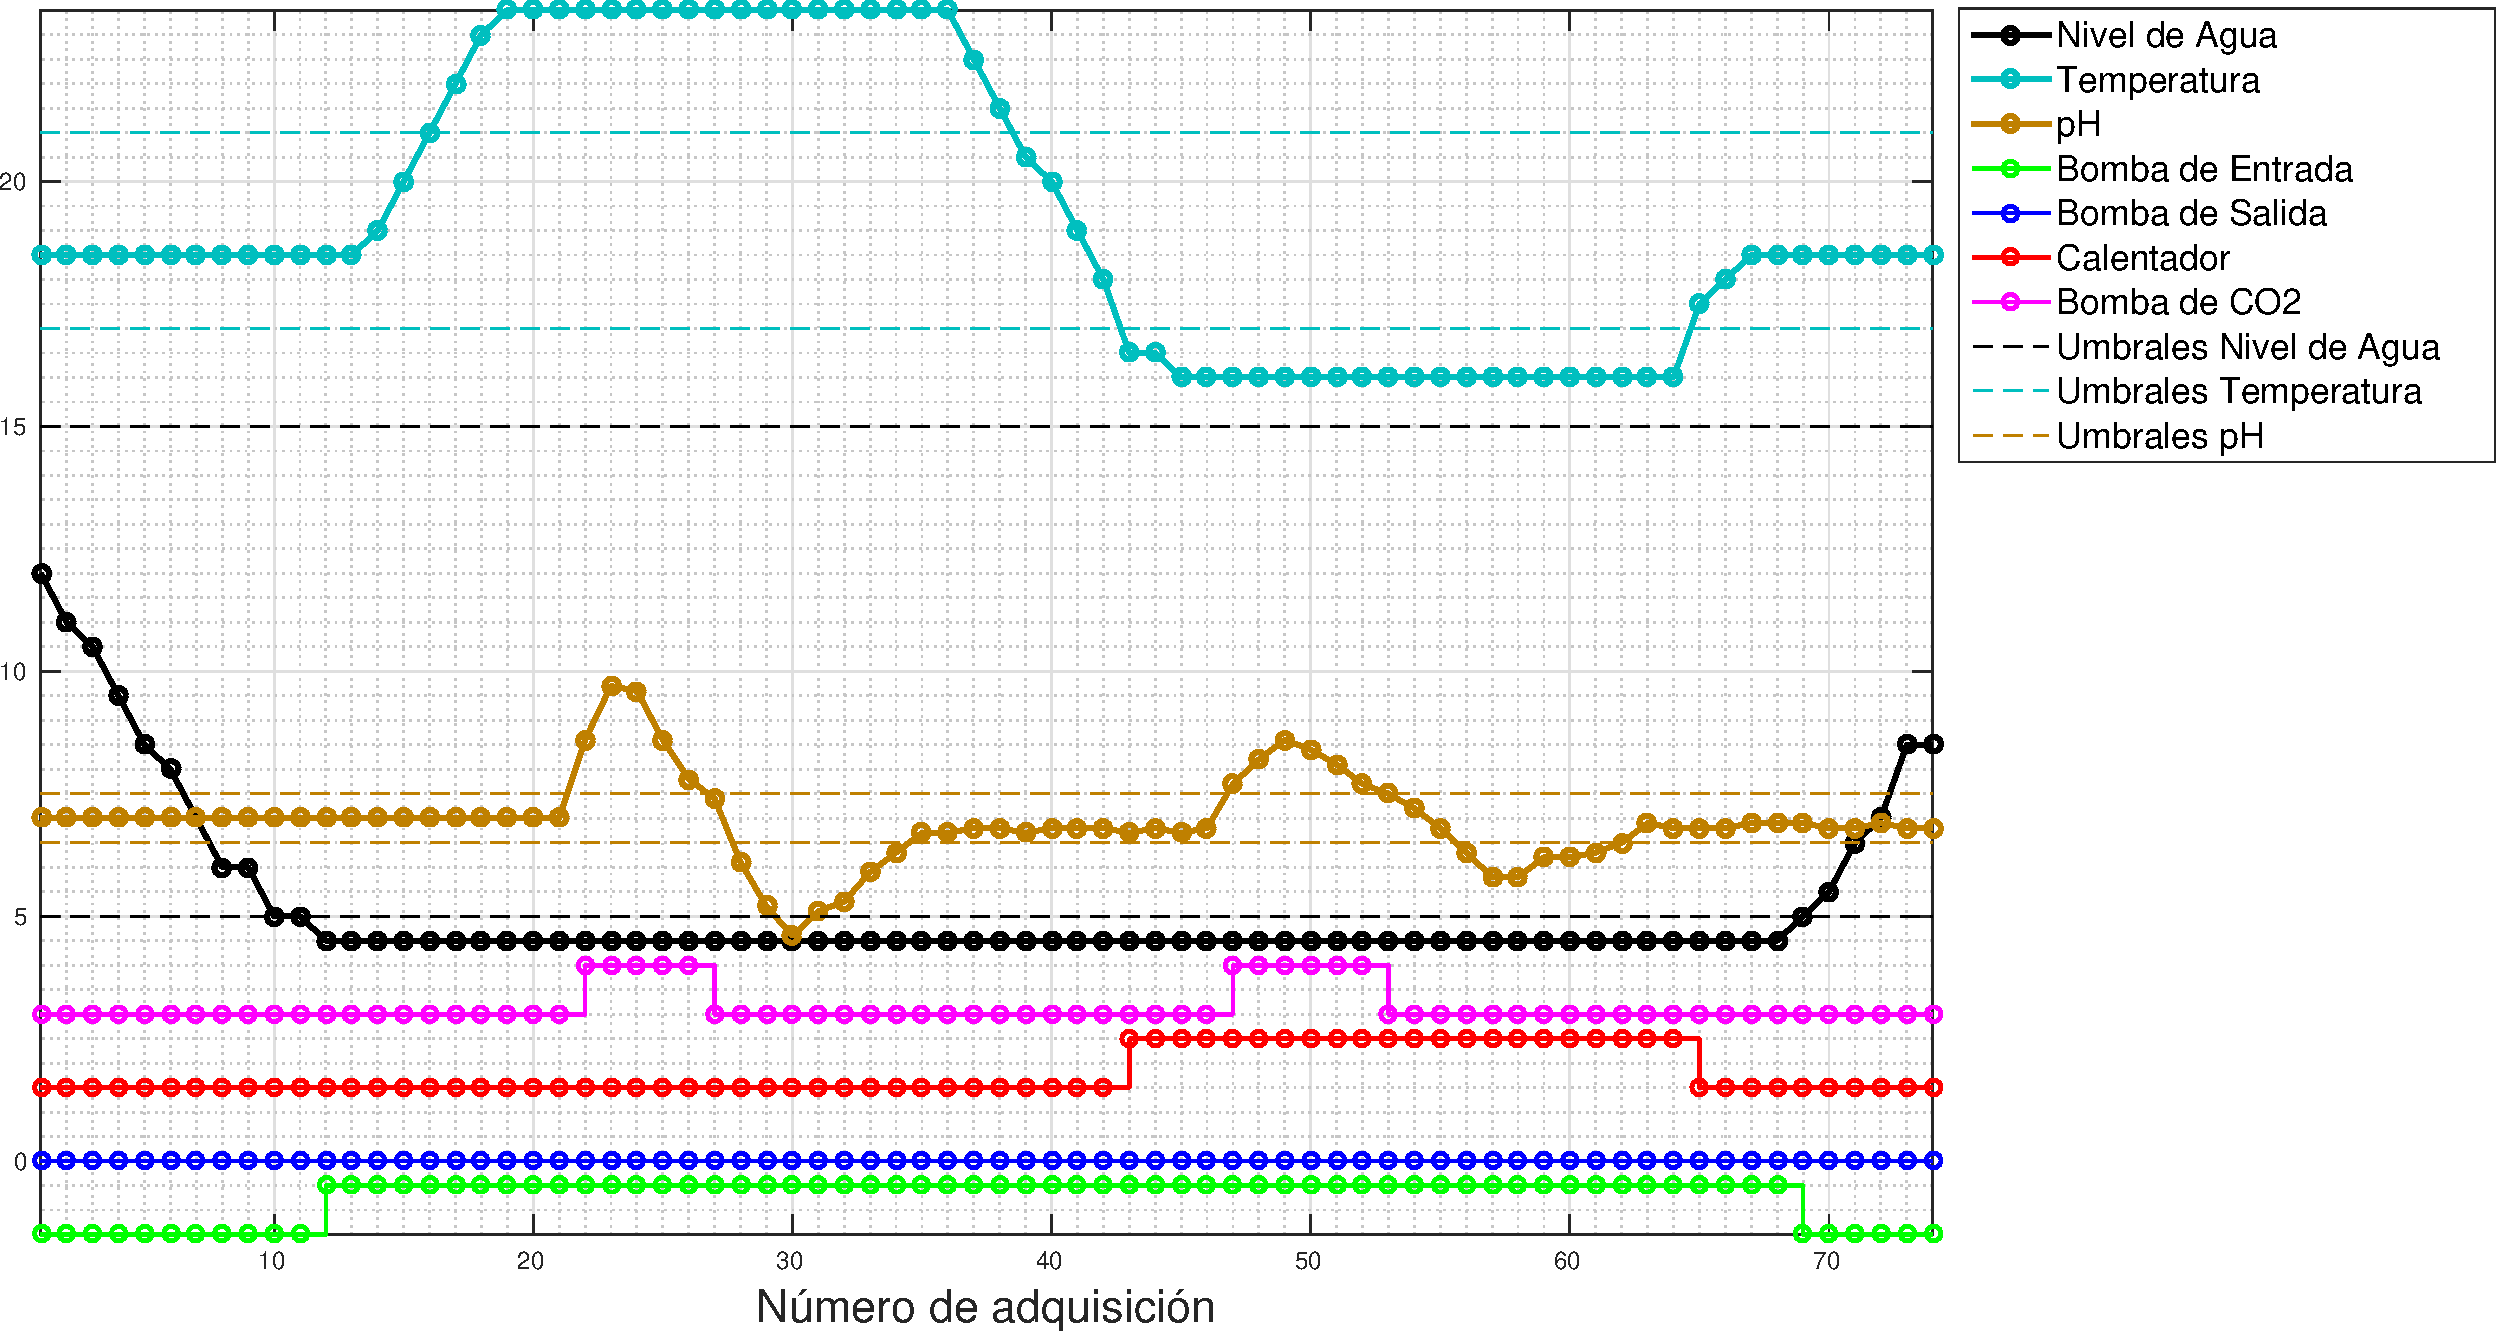
\includegraphics[width=\textwidth]{./Figures/plot3waterLow.pdf}
	\caption[Respuesta a tres alarmas simultáneas. Nivel de agua bajo y otras.]{Tres alarmas: nivel de agua bajo y otras.}
	\label{fig:alarma3WaterLow}
\end{figure}